\documentclass[11pt]{article}
\usepackage[T1]{fontenc}
\usepackage{lmodern}
\usepackage[margin=1in]{geometry}
\usepackage{microtype}
\usepackage{amsmath,amssymb}
\usepackage{graphicx}
\usepackage{booktabs,tabularx,array}
\usepackage{enumitem}
\usepackage{xcolor}
\usepackage[most]{tcolorbox}
\usepackage{caption}
\usepackage{upquote}
\usepackage{needspace}
\usepackage[colorlinks=true,linkcolor=blue!50!black,urlcolor=blue!50!black]{hyperref}

\definecolor{plainbg}{HTML}{EEF4FA}\definecolor{plainframe}{HTML}{2C6FA8}
\definecolor{warnbg}{HTML}{FBF1E6}\definecolor{warnframe}{HTML}{C07020}
\newtcolorbox{plain}[1][In plain terms]{colback=plainbg,colframe=plainframe,
  fonttitle=\bfseries\small,title={#1},boxrule=0.5pt,arc=2pt,left=6pt,right=6pt,top=4pt,bottom=4pt}
\newtcolorbox{caution}[1][Watch out]{colback=warnbg,colframe=warnframe,
  fonttitle=\bfseries\small,title={#1},boxrule=0.5pt,arc=2pt,left=6pt,right=6pt,top=4pt,bottom=4pt}
\newcommand{\code}[1]{\texttt{\small #1}}
\setlist{itemsep=2pt,topsep=4pt}
\renewcommand{\arraystretch}{1.15}
\captionsetup{font=small,labelfont=bf}
% primitive \input is expandable, so table rows that start with \multicolumn work
\makeatletter\let\rawinput\@@input\makeatother

\title{\textbf{Posterior inference from the 3\,$\times$\,80,000 run}\\[4pt]
\large Convergence, results, and what it means for the simulation study's truth}
\date{October 2026}
\author{}

\begin{document}
\maketitle
\vspace{-2.2em}

\begin{plain}[Summary]
The simulation study takes its ``true'' parameter values from the posterior shipped with the package, which came from a run of 3 chains $\times$ 10,000 iterations that had not fully converged. A much longer run, 3 chains $\times$ 80,000 iterations, has now been analysed. It \textbf{has converged}: every parameter has split R-hat below 1.006 and effective sample size above 700. Its answers \textbf{agree closely with the shipped values}: every shipped median lies within 0.27 posterior standard deviations of the 80k estimate, and most of the gaps are no larger than the sampling noise expected from the shipped file's 252 draws. So the simulation's truth values are sound: switching them to the 80k values would move none by more than 0.33 posterior standard deviations. The one result that does change is a credible interval: the female rate ratio's 95\% interval now includes 1.
\end{plain}

%=====================================================================
\section{Where the simulation's truth values come from}

The function \code{sim\_truth()} in \code{simulation/sim\_truth.R} reads \code{data/fitted\_posterior.rds}. That file holds 252 draws: the shipped run of 3 chains $\times$ 10,000 iterations, with the first third of each chain discarded and the rest thinned to every 80th draw. \code{sim\_truth()} takes the \textbf{posterior median of each parameter} across those 252 draws, giving one parameter vector: the rate-curve coefficients $\theta$, the noise-curve coefficients $\nu$, $\mu_b$, $\gamma$, $\sigma_\alpha$, $\psi$, $\sigma_\delta$, $\varphi$ and $\sigma_b$. The \code{fitted} scenario uses that vector unchanged. The other three scenarios change one piece of it.

Derived truths, such as the transit budget or the cure fractions, are computed from that median vector. This is a ``plug-in'' truth. It is internally consistent, because every derived quantity comes from the same set of parameters, but it is not identical to the posterior median of the derived quantity itself. The differences are small and do not affect the simulation, which only needs one coherent set of true values.

\begin{plain}
Yes, the simulation's truth is just the middle value of each parameter from the shipped fit. Your concern is the right one to have: if that fit had not settled down, its middle values could be in the wrong place, and the simulation would be testing the model against a slightly arbitrary world.
\end{plain}

%=====================================================================
\section{The 80k run and how it was checked}

\paragraph{Same model, same data.} The 80k fit, \code{results\_80k/infer\_fit.rds}, uses the identical data (1,101 subjects, 3,393 scans), identical settings and identical spline bases to the shipped fit. It ran for about 7 hours. All draws are finite and the pinned coefficient $\theta_1$ is constant, as it should be.

\paragraph{Burn-in.} The first third of each chain is discarded, the same rule the package uses everywhere, leaving 53,334 draws per chain and 160,002 in total. The trace plots in Figure~\ref{fig:traces} show the chains have left their starting values within the first few thousand iterations, well inside the discarded part.

\paragraph{Diagnostics.} Four checks, computed with the \code{posterior} package:

\begin{itemize}
  \item \textbf{Rank-normalised split R-hat} (Vehtari et al., 2021). It splits each chain in half and compares all six halves, after converting draws to ranks so heavy tails cannot hide a problem. The usual standard is below 1.01.
  \item \textbf{Classic R-hat}, the version the package's \code{convergence()} prints, for continuity with the README.
  \item \textbf{Bulk effective sample size (ESS)}: how many independent draws the correlated chain is worth for estimating the centre of the posterior. The usual standard is at least 400.
  \item \textbf{Tail ESS}: the same for the 5\% and 95\% quantiles, which matter for credible intervals.
\end{itemize}

\begin{center}
\small
\begin{tabular}{@{}l c c@{}}
\toprule
Check & Result, worst parameter & Standard \\
\midrule
Split R-hat & 1.0052, $\varphi_1$ & below 1.01 \\
Classic R-hat & 1.0024 & below 1.01 \\
Bulk ESS & 714, $\gamma_1$ & at least 400 \\
Tail ESS & 1,958, $\gamma_1$ & at least 400 \\
\bottomrule
\end{tabular}
\end{center}

All 31 monitored parameters pass all four checks. The per-chain medians of the slowest parameters agree to the third decimal place, and so do medians taken from the early, middle and late portions of the kept draws, so there is no sign of drift.

\paragraph{How long is long enough?} Figure~\ref{fig:conv} repeats the diagnostics using only the first $L$ iterations of each chain. Using only the first 10,000, the length of the shipped run, the worst split R-hat is 1.147, 13 of 31 parameters exceed 1.01, and the smallest bulk ESS is 16. The worst R-hat first drops below 1.01 at 40,000 iterations and the ESS standard between 40,000 and 60,000. This confirms your suspicion: 10,000 iterations was not enough for this model.

\begin{figure}[h]
\centering
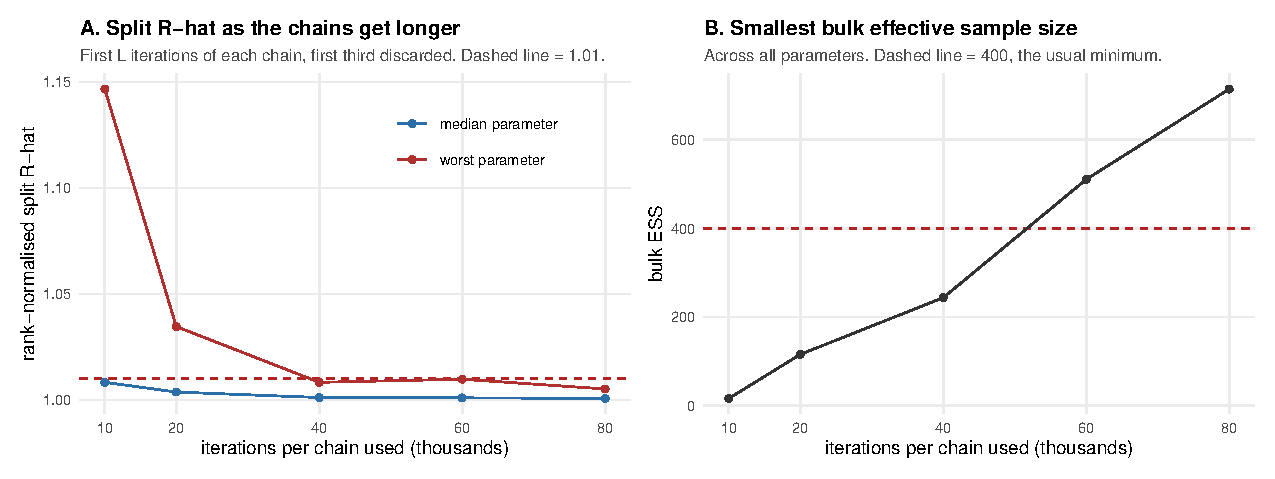
\includegraphics[width=\textwidth]{fig1_convergence.pdf}
\caption{Convergence as a function of chain length, recomputed from the first $L$ iterations of the 80k run. At 10,000 iterations the slowest parameters are far from converged; by 80,000 every check passes comfortably.}
\label{fig:conv}
\end{figure}

\begin{caution}[A caveat about the 10,000-iteration numbers]
The shipped file keeps only 252 pooled draws, not its chains, so the shipped run's own R-hat cannot be recomputed. The 10,000-iteration figures above come from the first 10,000 iterations of the \emph{80k} run. That is the same model, data and sampler at the same length, so it is a fair stand-in, but it is not literally the shipped run.
\end{caution}

\begin{figure}[h]
\centering
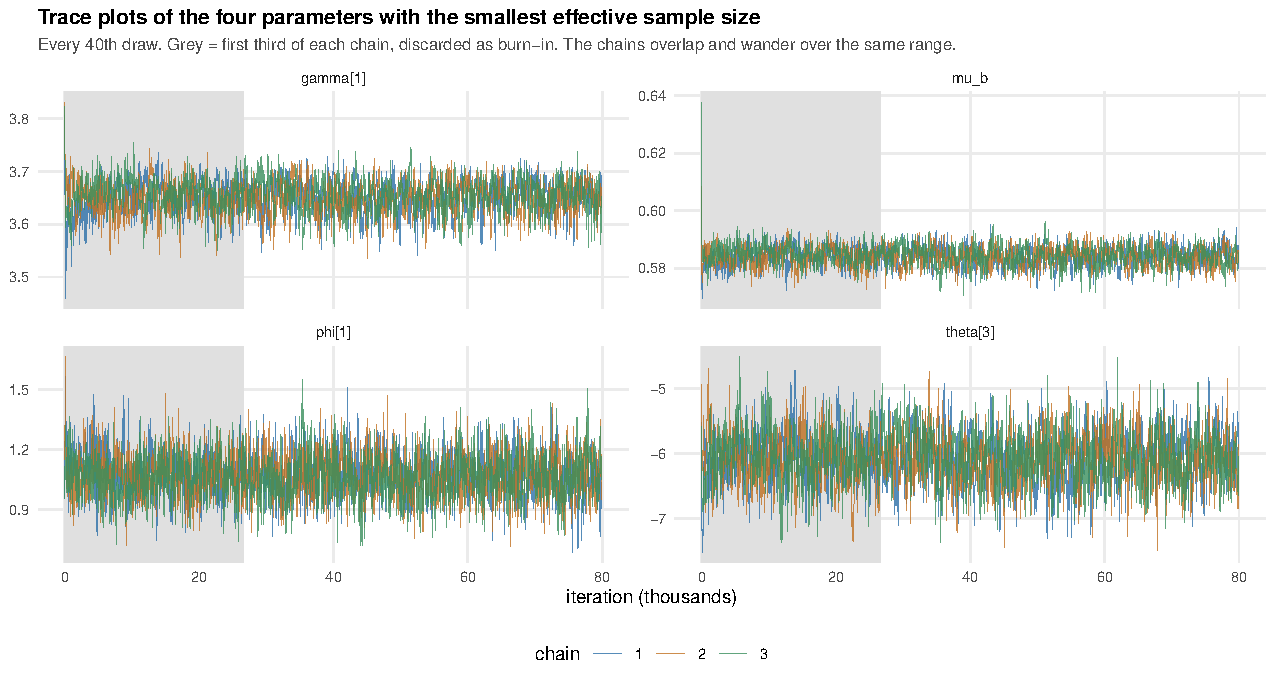
\includegraphics[width=\textwidth]{fig2_traces.pdf}
\caption{The four slowest-mixing parameters. The intercepts of the onset and susceptibility models and the floor move slowly, which is why they need long chains, but all three chains explore the same region throughout the kept draws.}
\label{fig:traces}
\end{figure}

\begin{plain}
MCMC works by sending three random walkers through the space of plausible answers. If they have run long enough, they should all be wandering over the same ground; R-hat measures whether they are, and ESS measures how much genuinely new information the wandering has collected. After 10,000 steps the walkers had not yet mixed for a handful of parameters. After 80,000 they have, by a comfortable margin.
\end{plain}

%=====================================================================
\section{Posterior results from the 80k run}

Posterior medians with 95\% credible intervals, on the scales the report uses. Covariates are centred, so intercepts refer to the cohort average. Crossing ages are computed within draw by the package's \code{crossing\_ages()} from 200 posterior draws of each run. Every other 80k quantity uses a random 20,000 of its 160,002 draws; shipped quantities use all 252.

\begin{center}
\small
\begin{tabularx}{\textwidth}{@{}X l l@{}}
\toprule
Quantity & 80k run & Shipped (3\,$\times$\,10k) \\
\midrule
\rawinput tab_results.tex 
\bottomrule
\end{tabularx}
\end{center}

The substantive picture is unchanged. APOE4 acts strongly on whether people accumulate (odds ratio about 5.4) and on when they start (time ratio 0.73, about 27\% earlier), and its effect on speed covers 1. Non-carriers cross the positivity threshold about 12.4 years later than carriers. Classifying subjects at a posterior probability of 0.5, 776 of 1,101 are accumulators in the 80k run, against 783 in the shipped one.

\begin{caution}[One conclusion changes: the female rate ratio]
The README reports the female rate ratio as 0.903 [0.811, 0.996], an interval that excludes 1, which would read as ``women accumulate about 10\% more slowly''. In the converged run it is 0.909 [0.810, 1.021], which \emph{includes} 1. The female odds ratio for ever accumulating, 1.45 [1.01, 2.08], now only just excludes 1. Neither estimate moved much; what changed is the upper end of the interval. The shipped intervals are 2.5\% and 97.5\% quantiles of only 252 draws, about 6 draws in each tail, so their endpoints are imprecise. Results that sit at the edge of significance should be reported from the 80k run.
\end{caution}

%=====================================================================
\section{Comparison with the values the simulation uses}

\subsection{Parameter by parameter}

For every parameter, the gap between the shipped median and the 80k median was measured in units of the 80k posterior standard deviation. This puts every parameter on the same scale: a gap of 1 would mean the shipped value is one full posterior SD away.

\begin{itemize}
  \item \textbf{All 31 monitored parameters} have gaps below 0.24 SD, and every shipped median lies inside the 80k 95\% interval.
  \item \textbf{The reported quantities}, shown in Figure~\ref{fig:shift}, have gaps below 0.27 SD.
\end{itemize}

\paragraph{Are these gaps real or noise?} A median estimated from 252 correlated draws carries Monte Carlo error. Measured in 80k posterior SDs, that error is about 0.08 to 0.10 SD for a typical parameter and up to 0.18 SD for the slowest. The 80k medians are far more precise, at most 0.04 SD. Dividing each gap by the shipped median's Monte Carlo error gives a typical value of 0.84, and 28 of 31 parameters fall under 2. The three just above 2 are $\varphi_1$, its transform $\pi$, and one rate-curve coefficient, $\theta_7$, all at about 2.3. With 31 comparisons, a few values near 2 are expected by chance. The gaps are therefore almost entirely the shipped file's sampling noise, not a systematic error from non-convergence.

\begin{figure}[h]
\centering
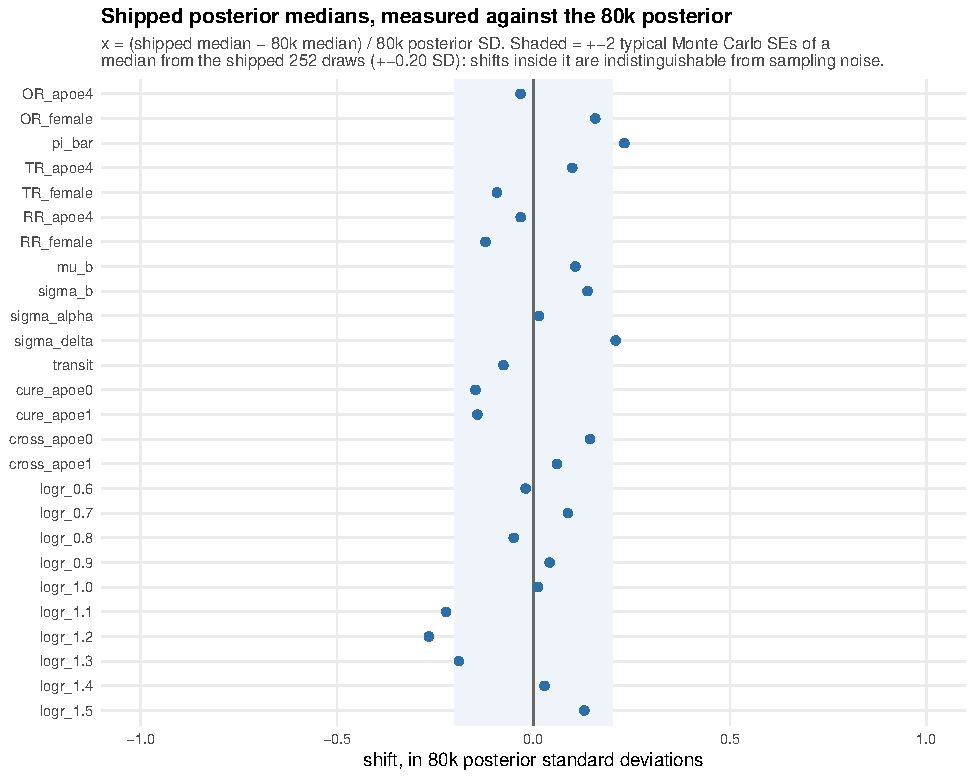
\includegraphics[width=0.78\textwidth]{fig3_shift.pdf}
\caption{Each dot is a reported quantity: how far the shipped median sits from the 80k median, in 80k posterior standard deviations. All are within $\pm 0.3$ SD; most lie inside the shaded band, which marks the size of gap that Monte Carlo noise alone produces.}
\label{fig:shift}
\end{figure}

\Needspace{18\baselineskip}
\subsection{What would change in the simulation}

Running \code{sim\_truth("fitted")} on the 80k draws instead of the shipped ones gives the truths below. The last column is the change, 80k minus shipped, in 80k posterior SDs.

\begin{center}
\small
\begin{tabular}{@{}l r r r@{}}
\toprule
Truth value & Shipped & 80k & Change, SD \\
\midrule
\rawinput tab_truth.tex 
\bottomrule
\end{tabular}
\end{center}

The largest change is 0.33 SD, for the rate curve at 1.2 SUVR. Every other change is a quarter of a posterior SD or less. For comparison, the simulation is designed to detect biases and coverage failures in the model's estimates, and the smallest of those that matters is on the order of the posterior SD itself. Truth values that move by a fraction of that do not change what the simulation can find.

\begin{plain}
The shipped fit had not fully settled, but it was already in the right place. Its middle values sit almost exactly where the much longer, properly converged run puts them, and the small differences are about what you would expect from estimating a middle value from only 252 draws. The simulation is testing the model against a realistic world either way.
\end{plain}

%=====================================================================
\section{Recommendations}

\begin{enumerate}
  \item \textbf{Report results from the 80k run.} It is the converged posterior, and it changes one interval-based conclusion, the female rate ratio.
  \item \textbf{The simulation can keep its current truth.} Changing it would move no truth value by more than a third of a posterior SD. If you prefer the truth to come from the converged run, save the pooled 80k draws in the same format as \code{data/fitted\_posterior.rds} and point \code{sim\_truth()} at that file. The code already accepts any matrix of draws through its \code{post} argument.
  \item \textbf{Treat 40,000 iterations per chain as a minimum} for future fits of this model. The slowest parameters, $\gamma_1$, $\mu_b$ and $\varphi_1$, need it.
\end{enumerate}

%=====================================================================
\section{Reproducing this analysis}

Run from the project root. Each script saves its outputs in \code{posterior\_80k/}.

\begin{center}
\small
\begin{tabularx}{\textwidth}{@{}l X@{}}
\toprule
Script & What it does \\
\midrule
\code{00\_load.R} & Loads the model code. Takes only function definitions from \code{run\_model.R}, because that file currently ends with interactive code that cannot be sourced. \\
\code{01\_convergence.R} & R-hat and ESS for every parameter, and by chain length. Writes \code{convergence\_80k.csv}. \\
\code{02\_summaries.R} & Posterior summaries, crossing ages, comparison with the shipped fit, and the implied simulation truth. Writes three CSV files. About 5 minutes. \\
\code{03\_figures.R} & Monte Carlo error of the medians, and the three figures. \\
\code{04\_tables.R} & The two tables in this report, generated from the CSV files. \\
\bottomrule
\end{tabularx}
\end{center}

\begin{verbatim}
for (s in sprintf("posterior_80k/%02d_%s.R", 1:4,
                  c("convergence", "summaries", "figures", "tables")))
  system2("Rscript", s)
\end{verbatim}

\end{document}
